\begin{center}
	\Huge
	Tangentens ligning og ekstrema
\end{center}

\section*{Tangentligningen}
\stepcounter{section}

Hældningen for tangenten til en funktion $f$ i et punkt $x_0$ kan vi som bekendt finde ved at differentiere $f$
og udregne $f'(x_0)$. Vi kan finde hele ligningen for tangenten ved at bruge punktet og forskriften for $f$. Lad os betragte et eksempel
\begin{exa}
	Vi får givet andengradspolynomiet $f$ givet ved
	\begin{align*}
		f(x) = 4x^2-5x+7
	\end{align*}
	og ønsker at bestemme tangentens ligning i punktet $(2,f(2))$. Det første, vi gør er at differentiere 
	funktionen
	\begin{align*}
		f'(x) = 8x - 5.
	\end{align*}
	Vi indsætter nu $x_0 = 2$ og får tangenthældningen
	\begin{align*}
		f'(2) = 8\cdot 2 - 5 = 11.
	\end{align*}
	Vores tangentligning må altså være på formen
	\begin{align}\label{eq:tangent}
		y = 11x + b,
	\end{align}
	og vi skal altså finde $b$. Vi ved, at $f$ skærer gennem punktet $(2,f(2))$, så vi bestemmer $f(2)$.
	\begin{align*}
		f(2) = 4\cdot 2^2-5\cdot 2 + 7 = 13.
	\end{align*}
	Vi kan nu indsætte dette i \eqref{eq:tangent} og løse for $b$.
	\begin{align*}
		y = 11x + b \ &\Leftrightarrow \ 13 = 11\cdot 2 + b \\
		&\Leftrightarrow	 \ 13 - 22 = b \\
		&\Leftrightarrow	 \ b = -9.
	\end{align*}
	Dette giver os derfor tangentligningen 
	\begin{align*}
		y = 11x-9.
	\end{align*}
	Vi tegner grafen for funktionen samt tangenten i et koordinatsystem på Figur \ref{fig:tangent}
	\begin{figure}[H]
		\centering
		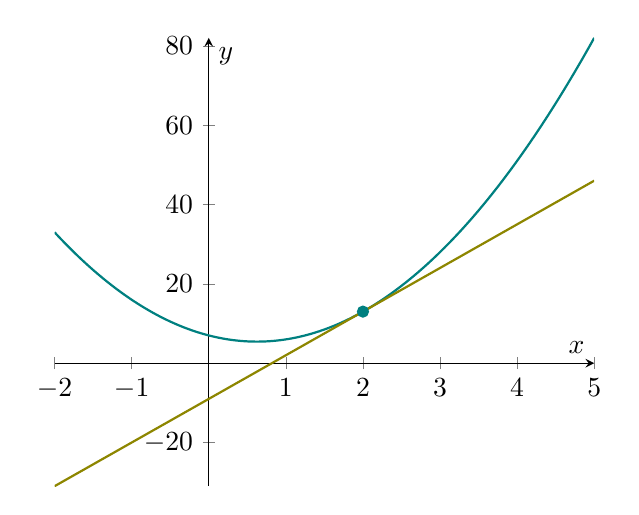
\begin{tikzpicture}
		\begin{axis}[
			axis lines = center,
			xmin = -2, xmax = 5,
			xlabel = $x$, ylabel = $y$, 
		]
			\addplot[color = teal, thick, domain = -2:5, samples = 400] {4*x^2-5*x+7};
			\addplot[color = olive, thick, domain = -2:5, samples = 100] {11*x-9};
			\filldraw[color = teal] (axis cs: 2,13) circle (2pt);
		\end{axis}
		\end{tikzpicture}
		\caption{Graf for $f$ samt tangent i punktet $(2,f(2))$}
		\label{fig:tangent}
	\end{figure}
	\phantom{h}
\end{exa}
Vi kan opskrive denne fremgangsmåde for at finde tangentligninger som en mere generel algoritme:
\begin{center}
	\textbf{Find ligning for tangent for $f$ i punktet $(x_0,f(x_0)).$}
\end{center}
\begin{enumerate}
	\item Bestem forskriften for den afledede funktion $f(x)$.
	\item Udregn tangenthældningen $a = f'(x_0)$.
	\item Udregn funktionsværdien $f(x_0)$.
	\item Indsæt tangenthældningen $a$ samt punktet $(x_0,f(x_0))$ i tangentens ligning, så
	\begin{align*}
		y = ax + b
	\end{align*}
	bliver til
	\begin{align}\label{eq:tangentalgo}
		f(x_0) = ax_0 + b.
	\end{align}
	\item Isolér $b$ i tangentligningen \eqref{eq:tangentalgo}.
	\item Opskriv tangentligningen $y = ax + b$ med de fundne værdier for $a$ og $b$.
\end{enumerate}

Det er også muligt at bestemme tangentens ligning ved at anvende en formel.
\begin{setn}\label{setn:tangent}
	For en differentiabel funktion $f$ er tangentens ligning i punktet $(x_0,f(x_0))$ givet ved
	\begin{align*}
		y = f'(x_0)\cdot(x-x_0) + f(x_0)
	\end{align*}
\end{setn}
\begin{proof}
	Opgave.
\end{proof}
Vi kan illustrere tangentens ligning på Figur \ref{fig:tangentligning}
\begin{figure}[H]
	\centering
	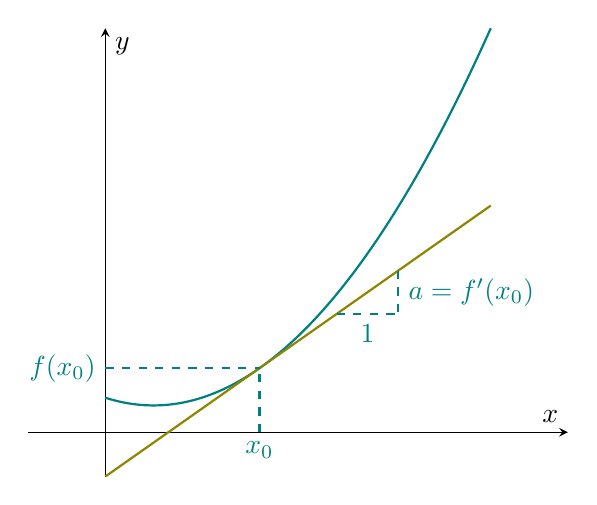
\begin{tikzpicture}
	\begin{axis}[
		axis lines = center,
		xmin = -1, xmax = 6,
		xlabel = $x$, ylabel = $y$, 
		ticks = none
		]
			\addplot[color = teal, thick, domain = 0:5, samples = 400] {4*x^2-5*x+7};
			\addplot[color = olive, thick, domain = 0:5, samples = 100] {11*x-9};
			\draw[color = teal, dashed, thick] (axis cs: 2,0) -- (axis cs: 2,13);
			\draw[color = teal, dashed,thick] (axis cs: 0,13) -- (axis cs: 2,13);
			\node[color = teal, anchor = north] at (axis cs: 2,0) {$x_0$};
			\node[color = teal, anchor = east] at (axis cs: 0,13) {$f(x_0)$};
			\draw[color = teal, dashed, thick] (axis cs: 3,24) -- (axis cs: 3.8,24)
			node[midway, anchor = north] {1};
			\draw[color = teal, dashed, thick] (axis cs: 3.8,32.8) -- (axis cs: 3.8,24)
			node[midway, anchor = west] {$a = f'(x_0)$};
	\end{axis}
	\end{tikzpicture}
	\caption{Tangentens ligning}
	\label{fig:tangentligning}
\end{figure}
Vi kan lave samme eksempel som før nu med tangentens ligning.
\begin{exa}
	Vi betragter igen funktionen $f$ givet ved
	\begin{align*}
		f(x) = 4x^2-5x+7
	\end{align*}
	og ønsker at bestemme tangentens ligning gennem punktet $(2,f(2))$ ved brug af formlen
	\begin{align*}
		y = f'(x_0)(x-x_0) + f(x_0).
	\end{align*}
	Vi skal udregne tallene $f'(x_0)$ og $f(x_0)$. Først udregnes $f'(x_0)$.
	Vi differentierer først.
	\begin{align*}
		f'(x) = 8x - 5.
	\end{align*}
	Så indsættes $x_0 = 2.$
	\begin{align*}
		f'(2) = 11.	
	\end{align*}	 
	Vi bestemmer nu $f(2)$:
	\begin{align*}
		f(2) = 13.
	\end{align*}
	Disse tal indsættes i tangentens ligning
	\begin{align*}
		y &= f'(2)(x-2) + f(2)\\
		&= 11(x-2)+13\\
		&= 11x-22+13\\
		&= 11x-9.
	\end{align*}
	Vi får altså også her tangentens ligning til at være
	\begin{align*}
		y = 11x-9.
	\end{align*}
\end{exa}

Vi tilføjer nogle funktioner til vores tabel.
\begin{table}[H]
	\centering
	\rowcolors{1}{white}{teal!30}
	\begin{tabular}{cc}
		$f(x)$ & $f'(x)$ \\
		$k$ & $0$ \\
		$x$ & $1$ \\
		$ax + b$  & $a$ \\
		$x^2$ & $2x$ \\
		$x^a$ & $ax^{a-1} $ \\
		$\sqrt{x}$ & $\frac{1}{2\sqrt{x}}$ \\
		$\frac{1}{x}$ & $-\frac{1}{x^2}$ \\
		$\ln(x)$ & $\frac{1}{x}$ \\
	 	$e^x$ & $e^x$ \\
	 	$\cos(x)$ & $-\sin(x)$ \\
	 	$\sin(x)$ & $\cos(x)$ \\
	\end{tabular}
	\caption{Udvalgte afledede funktioner}
	\label{tab:afledt}
\end{table}

\section*{Ekstrema}
\stepcounter{section}

Vi talte i 1.g om ekstremumspunkter. Disse var punkter, der lokalt er maksimum eller minimum for en funktion. 

I mange sammenhænge er det en fordel at kunne bestemme \textit{toppunkter/maksima og minima} for en funktion $f$. Hvis $f$ er en differentiabel funktion, så kan vi udnytte differentialregning til at bestemme sådanne punkter. Et punkt, der enten er et maksimum eller et minimum kaldes et \textit{ekstremumspunkt}. 

Vi har følgende sætning:
\begin{setn}[Ekstremumspunkter]
	Lad $f$ være en differentiabel funktion. Hvis et punkt $P(x_0,f(x_0))$ er et ekstremumspunkt for $f$, så gælder der, at 
	\begin{align*}
		f'(x_0) = 0.
	\end{align*}
\end{setn}
Det er dog værd at bemærke, at vi ikke nødvendigvis har den omvendte implikation; hvis $f'(x_0)=0$, så er $(x_0,f(x_0))$ ikke nødvendigvis et ekstremumspunkt. Vi kalder sådanne for \textit{vandrette vendetangenter}. Vi kan se både en vandret vendetangent samt to ekstrema på Figur \ref{fig:ekstremavende}.


\begin{figure}[H]
	\centering
	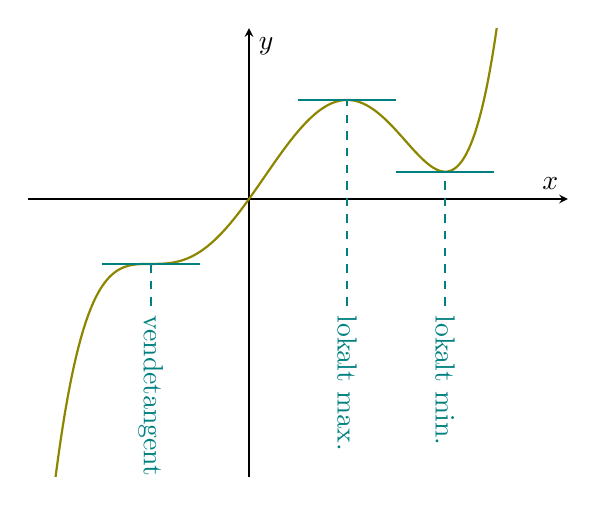
\begin{tikzpicture}
	\begin{axis}[
	axis lines = center, 
	xmin = -4.5, xmax = 6.5,
	ymin = -130, ymax = 80,
	xlabel = $x$, ylabel = $y$, 
	ticks = none,
	]
		\addplot[color = olive, thick, domain = -5:7, samples = 400] 
		{1/5*x^5-1/2*x^4-4*x^3+4*x^2+32*x };
		\node[color = teal, anchor = west, rotate = -90] at (axis cs: -2,-50) {vendetangent};
		\draw[color = teal, dashed, thick] (axis cs: -2,-50) -- (axis cs:-2,-152/5); 
		\node[color = teal, anchor = west, rotate = -90] at (axis cs: 2,-50) {lokalt max.};
		\draw[color = teal, dashed, thick] (axis cs: 2,-50) -- (axis cs:2,232/5); 
		\node[color = teal, anchor = west, rotate = -90] at (axis cs: 4,-50) {lokalt min.};
		\draw[color = teal, dashed, thick] (axis cs: 4,-50) -- (axis cs: 4,64/5); 
		\draw[color = teal, thick] (axis cs: -3,-152/5) -- (axis cs: -1,-152/5); 
		\draw[color = teal, thick] (axis cs: 1,232/5) -- (axis cs: 3,232/5); 
		\draw[color = teal, thick] (axis cs: 3,64/5) -- (axis cs: 5,64/5); 
	\end{axis}
	\end{tikzpicture}
	\caption{Forskellige ekstrema for en funktion samt vandrette tangenter}
	\label{fig:ekstremavende}
\end{figure}
\newpage
\begin{exa}
	Lad $f$ være givet ved
	\begin{align*}
		f(x) = x^3-6x^2+5.
	\end{align*}
	Vi ønsker at bestemme ekstrema for $f$. Vi differentierer derfor først $f$.
	\begin{align*}
		f'(x) = 3x^2-12x = 3x(x-4).
	\end{align*}
	Dette sættes nu lig $0$, og vi får
	\begin{align*}
		3x(x-4) = 0, 
	\end{align*}
	og ved hjælp af nulreglen ved vi, at $x=0$ eller $x = 4$. Vi bestemmer nu de tilhørende $y$-værdier og vi får
	\begin{align*}
		f(0) = 5
	\end{align*}
	og 
	\begin{align*}
		f(4) &= 4^3 - 6\cdot 4^2+5\\
		&= 64-96+5\\
		&= -27.
	\end{align*}
	Vi har derfor en vandret tangent i $P(0,5)$ og $Q(4,-27)$. For at bestemme, om det er et ekstremumspunkt, så tegner vi grafen. Denne kan ses af Figur \ref{fig:ekstrema}
	\begin{figure}[H]
		\centering
		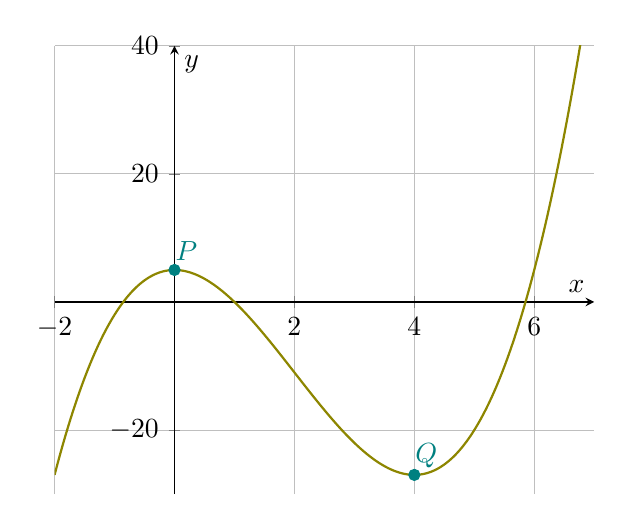
\begin{tikzpicture}
			\begin{axis}[axis lines = middle,
			xmin = -2, xmax = 7,
			ymin = -30, ymax = 40,
			xlabel = $x$, 
			ylabel = $y$,
			grid = both]
				\addplot[color = olive, samples = 200, domain = -2:7, thick] {x^3-6*x^2+5};
				\filldraw[color = teal] (axis cs:0,5) circle (2pt);
				\filldraw[color = teal] (axis cs:4,-27) circle (2pt);
				\node[color = teal] at (axis cs: 0.2,8) {$P$};
				\node[color = teal] at (axis cs: 4.2,-24) {$Q$};
			\end{axis}
		\end{tikzpicture}
		\caption{Graf for funktionen $f$.}
		\label{fig:ekstrema}
	\end{figure}
\end{exa}
Af Figur \ref{fig:ekstrema} kan vi se, at punkterne $P$ og $Q$ er ekstremumspunkter. $P$ er et \textit{lokalt maksimum} og $Q$ er et \textit{lokalt minimum}. Vi kan også se, at $f$ ikke har nogle 
\textit{globale ekstrema}.




\subsection*{Opgave 1}
\begin{align*}
&1) \ f(x) = x^2,\  P(-1,f(-1))  &&2) \   f(x)=2x^2-1x+3, \ P(0,f(0))    \\
&3) \ f(x) = \frac{1}{x} -x^3, \ P(2,f(2))   &&4) \ f(x) = \sqrt{x}, \ P(4,f(4))    \\
&5) \ f(x) = 7x+3,\ P(3,f(3))   &&6) \ f(x) = -3x^2+5x-1, \ P(1,f(1))     \\
&7) \ f(x) = 27, \ P(1000,f(1000))   &&8) \ f(x) = 3x^2-2\sqrt{x}, \ P(9,f(9))     \\
&9) \ f(x) = \frac{10}{x}+3x^3, \ P(2,f(2))   &&10) \ f(x) = 5x^3+2x^2+x+1, \ P(-2,f(-2))     \\
\end{align*}
	
\subsection*{Opgave 2}
Giv et bevis for Sætning \ref{setn:tangent}. Følg skridtene i tangentligningsalgoritmen før sætningen, men uden en given funktion.
	
	
\subsection*{Opgave 3}
Anvend, at $f(x) = x^a$ har differentialkvotienten $f'(x) = ax^{a-1}$ til at vise følgende
\begin{enumerate}[label=\roman*)]
	\item $f(x) = \frac{1}{x}$ har $f'(x) = -\frac{1}{x^2}$
	\item $g(x) = \sqrt{x}$ har $g'(x) = \frac{1}{2\sqrt{x}}$
\end{enumerate}

\subsection*{Opgave 4}

Bestem ekstremumspunkter for følgende funktioner. Løs først ligningen $f'(x)=0$ og tegn derefter grafen for funktionen.  Afgør til sidst, om der er tale om globale maksimum/minimum eller lokale maksimum/minimum.

\begin{align*}
	&1) \ -x^2+10    &&2) \  x^3     \\
	&3) \  x^4-8x^2   &&4) \ \ln(x) - \frac{1}{2}x^2      \\
	&5) \ 6\sqrt{x}-x^3    &&6) \   \frac{16}{x} +x^2    \\
	&7) \  x^5-10x^4   &&8) \ \frac{8}{x} + 2x      \\
\end{align*}

\subsection*{Opgave 5}
\begin{enumerate}[label=\roman*)]
	\item Tegn funktionen $\sin(x)$ på intervallet $[-10,10]$.
	\item Hvor mange ekstrema har $\sin(x)$ på dette interval og hvilken type har de?
	\item Bestem ekstrema for $\sin(x)$.
\end{enumerate}

\subsection*{Opgave 6}
\begin{enumerate}[label=\roman*)]
	\item Hvad sker der, hvis I differentierer $\cos(x)$ to gange?
	\item Hvad sker der, hvis I differentierer $\sin(x)$ to gange?
	\item Hvad sker der, hvis I differentierer $\cos(x)$ fire gange?
	\item Hvad sker der, hvis I differentierer $\sin(x)$ fire gange?
\end{enumerate}